% !TEX root = ../../thesis.tex

\section{Intertext Clients} \label{intertextClients}

Intertext clients are the user facing products of Intertext, that builds the bridge between the user and servers that serve IUIDL. They are meant to be implemented natively for the host platform in the most optimal way possible. 

For example, on mobile platforms such as iOS and Andriod, UI elements would be larger and more suitable for touch interactions. Primary interaction would be translated as "tap" while secondary interactions, if any, would be translated as "tap and hold". The layout would adjust itself based on the screen size. The client would be implemented with either native technologies such as Swift/Objective-C for iOS and Kotlin/Java for Android, or with hybrid technologies that gets compiled into native code, such as React Native or Flutter for maximum responsiveness and efficiency. 

At the time of this paper, a web client and a command-line client is implemented. Native clients for iOS and Android, and desktop clients for Mac OS, Windows and several Linux distributions are among the ones that are planned, more could be found in \nameref{futureWork} section.

Intertext clients consists of two main parts; components and commands. Each Intertext client implement these separately, based on the host platform and its capabilities. Each client also implements the  their own local storage, state management strategy, and communication technique with the server.

\subsection{Components}

Components are anything that has a visual representation. All component stem from a generic IUIDL definition, and is interpreted based on the host platform requirements. They can be organisational or presentational. Organisational components are the layout components, they are used to position presentational components on the screen. Intertext implements a version of css flexbox specification as a layout system, which could be used to implement responsive interfaces for all screen sizes. For non-browser based platforms, we use the popular Yoga layout engine, which is a standalone implementation of the css flexbox specification in C++, allowing us to target almost any platform. More details on the layout system is given in \nameref{implementation} section.

Most presentational Intertext components share a concept, "intent", which is a way to communicate the intention of the UI element based on its use-case. Intertext clients renders the UI elements differently based on its intent, allowing a way for the developer to convey an intention of an UI element to the user without being able to intercept with the styles. For instance, an error message could be shown in a block component that has the intent "error", and it will be rendered with a red background, indicating to the user that it is an error message. \ref{fig:intents} shows an example of intents on block component for Intertext web client.

\begin{figure}
  \centering
  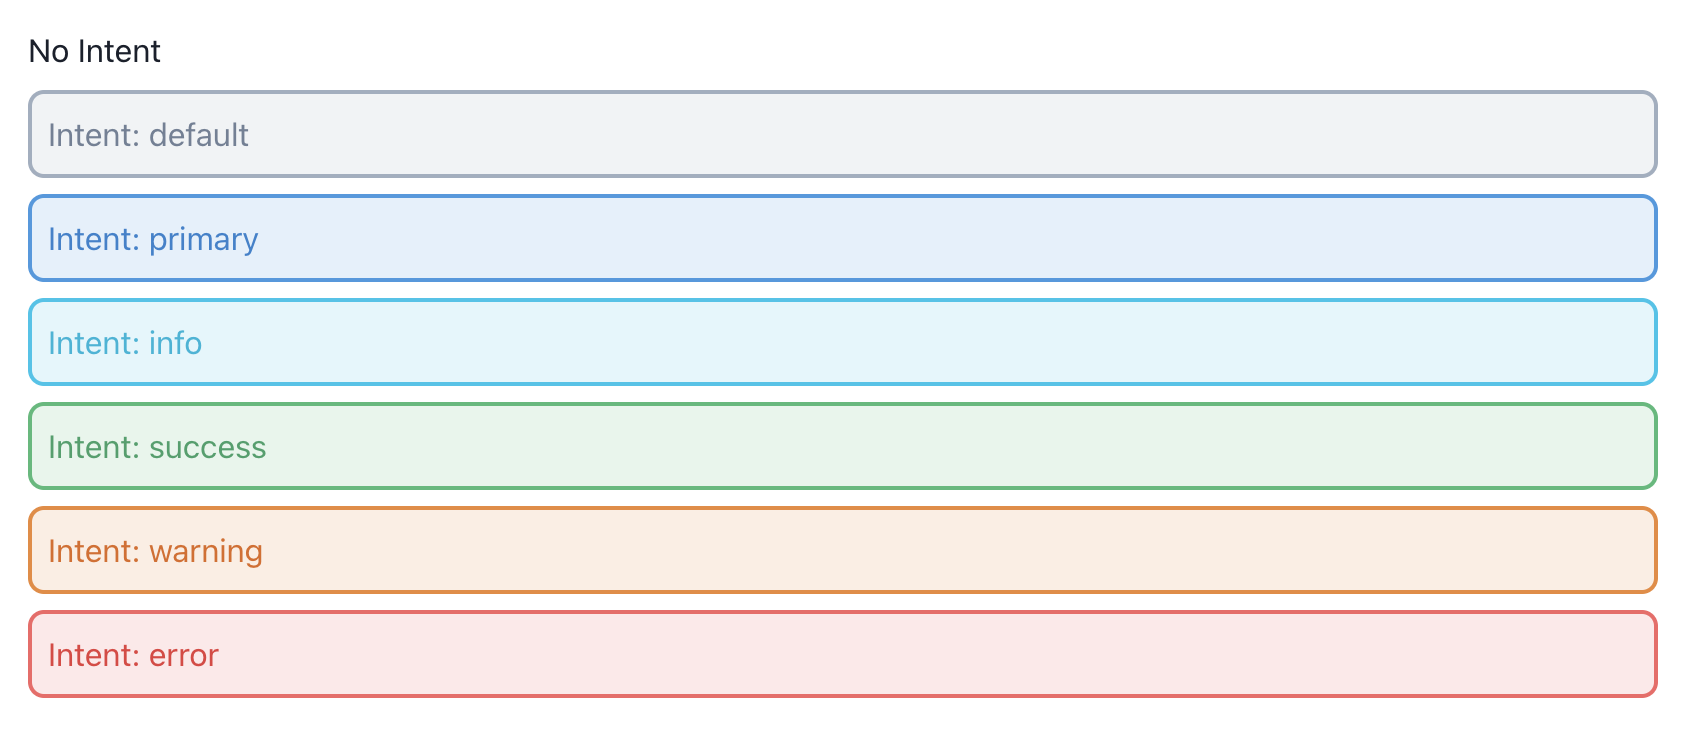
\includegraphics[width=13cm]{thesis/paper/images/intents.png}
  \caption{Intents for Block components}%
  \label{fig:intents}%
\end{figure}

\subsection{Commands}

Commands are IUIDL statements that are used to instruct Intertext client to take an action. These actions can be triggered upon interaction with some components (such as clicking a button or submitting a form), a life-cycle event, with a timeout, or on page load. Commands are very primitive by design, they are not meant to build application logic with. They are merely for asking the Intertext client to communicate with the server, store something, read something that is stored, or retrieve some user data. Command system is designed in order to ensure Intertext client is aware of what it is being asked to do, so that it can control and restrict the entire flow, ask for permission from the user when necessary, or simply refuse to take an action if needed. 

Figure \ref{fig:ex_cmd_post_timeout} shows an example of how a network request action can be executed upon a delay, and Figure \ref{fig:ex_cmd_form} shows how a form can be submitted with reference to input fields. More on commands will be on \nameref{implementation} section.

\begin{figure}
\begin{minipage}{\linewidth}
\begin{lstlisting}[language=xml]
<timeout delay="1000">
  <post endpoint="/refresh"></post>
</timeout>
\end{lstlisting}
\end{minipage}
\caption{Post command on Timeout}%
\label{fig:ex_cmd_post_timeout}%
\end{figure}

\begin{figure}
\begin{minipage}{\linewidth}
\begin{lstlisting}[language=xml]
<form endpoint="/todo/save">
  <input name="item_title"></input>
  <input name="item_description"></input>
  <button>Submit</button>
</form>
\end{lstlisting}
\end{minipage}
\caption{Form command with reference on server side to internal input values}%
\label{fig:ex_cmd_form}%
\end{figure}

\begin{figure}
\begin{minipage}{\linewidth}
\begin{lstlisting}[language=javascript]
router.get('/signup', async (req, res, next) => {
  
  const currentStep = req.body.state?.current_step ?? 0
  const currentFormData = req.body.params?.form_data
  const previousFormData = req.body.state?.form_data
  
  // check if user finished the form
  if (currentStep == LAST_STEP) {
    
    // execute signup logic
    const error = await signupUser(req.body.state?)
    
    // render success or error page based on
    // the signup result
    res.render(error
      ? 'signup_form_error'
      : 'signup_form_success',
    { error });
  
  } else {
    
    // render signup form
    res.render('signup_form', {
      // increment the current step
      step: currentStep + 1
      // merge current form data with previous
      formData: merge(previousFormData, currentFormData)
    });
  }
});
\end{lstlisting}
\end{minipage}
\caption{Handling a sign-up flow with multiple steps}%
\label{fig:state_signup_progress_js}%
\end{figure}

\subsection{State Management}

Intertext clients offer basic state management, making it possible to serve stateful Intertext applications using serverless/stateless backends. Front-end state can be fully driven from the backend via IUIDL. Intertext client offers two types of storage, persisted and volatile. 

Volatile storage is kept in the memory and it is persisted across the session. The purpose of this storage is to keep temporary values, such as users progress in a long form distributed across multiple pages. Intertext clients passes the entire application state on the volatile storage to the backend on every request, allowing backend to build logic around the current state of the front-end application, and serve the UI accordingly. Figure \ref{fig:state_signup_progress_js} and \ref{fig:state_signup_progress_xml} shows this through an hypothetical sign up form with steps distributed across multiple steps. On figure \ref{fig:state_signup_progress_js}, we see the pseudo-code implementation of the stateless backend for this scenario. It can be seen that the current step user is at on the form, and the form data collected thus far is kept in the volatile state on the front-end. The state gets passed on to the backend on every request made to the "/signup" endpoint. We retrieve the current step, and serve different responses accordingly. If user completed the last step, then we execute our application logic (which in this case is signing user up), and render the result page. Otherwise, we increment the current step, combine the form data collected thus far, and render the form template with these. On the form template on figure \ref{fig:state_signup_progress_xml}, we use the <state> block to instruct the Intertext client to record these new set of data to the front-end, so it could be passed on to the backend on the next request. Moreover, we render the correct form UI based on the step user is currently at.

Another type of storage is the persisted storage. As the name suggests, values stored this way is persisted across sessions. Unlike the volatile storage, in which the data is kept in the memory, persisted storage gets stored locally using the storage option available to the host platform. By default, data available in the persisted storage is not passed on to the backend in every request automatically, but can be configured to do so.

In order to protect user privacy, Intertext clients block cross-origin storage reads/writes, preventing users to be tracked across Intertext applications. In another words, state management is bound to the origin. Lets say "sub1.example.com" wrote data to the storage. This data can only be read or manipulated by the very same domain. "sub2.example.com" or "sub.example2.com" or any other domain will not have access to this data. While this behaviour protects users from cross-origin tracking, it may also inconvenience some users, especially in scenarios such as services that shares the same user login that is distributed across multiple domains/subdomains. As mentioned further in the \nameref{futureWork} section, we plan to add a feature where Intertext clients would ask for user permission to share data between domains/subdomains instead of directly blocking it.

\begin{figure}
\begin{minipage}{\linewidth}
\begin{lstlisting}[language=xml]
<!-- signup_form -->

<!-- set front-end state to read on later requests  -->
<state key="current_step">{{ step }}</state>
<state key="form_data">{{ formData }}</state>

{{#ifEquals step 1}}
  <!-- step 1 -->
{{/ifEquals}}

{{#ifEquals step 2}}
  <!-- form elements for step 2 -->
{{/ifEquals}}

<!-- ... -->
\end{lstlisting}

\begin{lstlisting}[language=xml]
<!-- signup_form_success -->

<h1 intent="success">Sign Up Successful!</h1>
<p intent="success">Please check your verification email</p>
\end{lstlisting}

\begin{lstlisting}[language=xml]
<!-- signup_form_error -->

<h1 intent="error">Something went wrong</h1>
<p intent="error">{{error}}</p>
\end{lstlisting}

\end{minipage}
\caption{Template files for multi-step sign up flow at Figure \ref{fig:state_signup_progress_js}}%
\label{fig:state_signup_progress_xml}%
\end{figure}
